\chapter{init Linux}
\section{Script de démarrage}

Au démarrage, le système exécute les scripts situés dans \textbf{/etc/init.d/} :

\begin{center} 
\hspace{15cm}
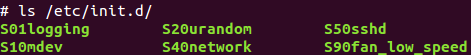
\includegraphics[width=10cm]{init_d.png}
\end{center}
\vspace{0.5cm}

\subsection{S01logging}

Ce script va exécuter les programmes suivants :

\begin{itemize}
	\item /sbin/syslogd
	\item /sbin/klogd
\end{itemize}

Version de \textbf{syslogd} : BusyBox v1.22.1 (2015-04-16 16:07:35 CEST) multi-call binary.\\
Version de \textbf{klogd} :BusyBox v1.22.1 (2015-04-16 16:07:35 CEST) multi-call binary.

Je n'ai trouvé aucune information sur des vulnérabilités possibles à propos de BusyBox v1.22.1 (des infos existent pour les versions antérieures de BusyBox, mais plus aucune à partir de la version 1.21).

\subsection{S10mdev}

Ce script va exécuter le programme suivant :

\begin{itemize}
	\item /sbin/mdev
\end{itemize}

Version de \textbf{mdev} : BusyBox v1.22.1 (2015-04-16 16:07:35 CEST) multi-call binary.

Je n'ai trouvé aucune information sur des vulnérabilités possibles à propos de BusyBox v1.22.1.

\subsection{S20urandom}

Ce script ne lance aucun exécutable. Cependant il va simplement sauvegarder la \textbf{random seed} lors de l'arrêt du système et la recharger à son démarrage.

Une version du script est donnée : \textbf{Version:	(\#)urandom  1.33  22-Jun-1998  miquels@cistron.nl}

\subsection{S40network}

Ce script va exécuter les programmes suivants :

\begin{itemize}
	\item /sbin/ifup (au démarrage du système)
	\item /sbin/ifdown (à l'arrêt du système)
\end{itemize}

Version de \textbf{ifup} : BusyBox v1.22.1 (2015-04-16 16:07:35 CEST) multi-call binary.

Je n'ai trouvé aucune information sur des vulnérabilités possibles à propos de BusyBox v1.22.1.

\subsection{S50sshd}

Ce script va exécuter le programme suivant :

\begin{itemize}
	\item /usr/sbin/sshd
\end{itemize}

Version de \textbf{sshd} : OpenSSH\_6.7p1, OpenSSL 1.0.1j 15 Oct 2014

Ces versions de OpenSSH et OpenSSL sont listées pour un certain nombre de vulnérabilités sur les sites indiqués dans la donnée. En revanche je n'ai pas trouvé d'informations pour éviter ces problèmes.

\subsection{S90fan\_low\_speed}

Ce script ne lance aucun exécutable. Il va écrire dans des fichiers du système qui permettent de contrôler le ventilateur.

\section{Démons}
La liste des démons qui doivent être démarrés se trouve dans le fichier \textbf{/etc/inittab} qui décrit également quand et comment ils doivent être démarrés. Par exemple au démarrage du système, à l'arrêt du système, ...\\

\subsection{Contrôle des droits de daemon2}

Généralement les démons sont démarrés en mode \textbf{root}. Mais dans le programme du démon, on peut utiliser les appels systèmes \textbf{umask()}, \textbf{setsid()}, \textbf{setegid()} et \textbf{seteuid()} pour changer les droits du processus (démon) afin qu'il n'ait plus les droits \textbf{root} pour éviter qu'un attaquant puisse se servir du démon pour faire des choses en tant que \textbf{root}. \\

Dans ce la labo, le code source d'un démon était donné (daemon2.c). Il a fallu le compiler (\textbf{./buildroot/output/host/usr/bin/arm-linux-gnueabihf-gcc daemon2.c -o daemon2}
) pour la carte Odroid et copier l'exécutable sur la carte (directement dans \textbf{/home/}). \\

Ensuite il a fallu contrôler les droits du démon. Pour ce faire il à déjà fallu créer un utilisateur nommé \textbf{test} ainsi que le répertoire \textbf{/home/test/daemon/}.\\

Pour tester les droits, la première fois on a créé ce répertoire en tant qu'utilisateur \textbf{root}. Puis on à lancé le démon, et on a vérifié si il s'est exécuté correctement ou non avec le fichier \textbf{/var/log/messages}

\begin{center} 
\hspace{15cm}
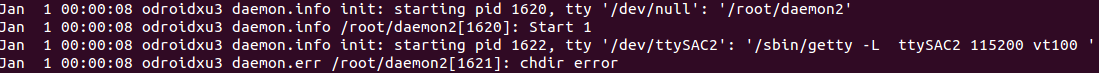
\includegraphics[width=16cm]{daemon_messages_1.png}
\end{center}
\vspace{0.5cm}

et les commandes \textbf{ps -ale | grep daemon}, \textbf{plsof | grep daemon} et \textbf{ls -lisa /home/test/daemon}

\begin{center} 
\hspace{15cm}
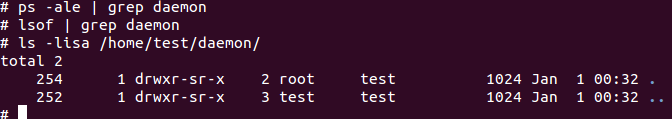
\includegraphics[width=16cm]{daemon_ps_lsof_txt_1.png}
\end{center}
\vspace{0.5cm}

Cela nous a permis de constater que le démon n'a pas pu se lancer correctement (il n'est pas dans les processus en cours d'exécution) et que c'est parce qu'il n'a pas pu créer le fichier \textbf{t.txt} dans le répertoire. Le fichier \textbf{messages} nous indique aucune erreur dans le lancement du démon, et si on regarde le code du démon, c'est qu'il a réussi à accéder au répertoire \textbf{/home/test/daemon} (avec la commande \textbf{chdir}) mais qu'il n'a pas pu créer et ouvrir le fichier \textbf{t.txt}, probablement parce qu'il n'a pas les droits nécessaires.\\

Ensuite on a supprimé ce répertoire \textbf{/home/test/daemon/} et on l'a recréé mais en tant qu'utilisateur \textbf{test}, et on a relancé le démon.\\

Cette fois-ci le programme redémarre et s'exécute normalement, comme on peut le voir dans les processus :

\begin{center} 
\hspace{15cm}
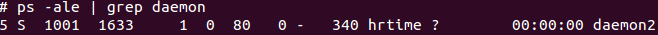
\includegraphics[width=16cm]{daemon_ps_2.png}
\end{center}
\vspace{0.5cm}

les fichiers ouverts :

\begin{center} 
\hspace{15cm}
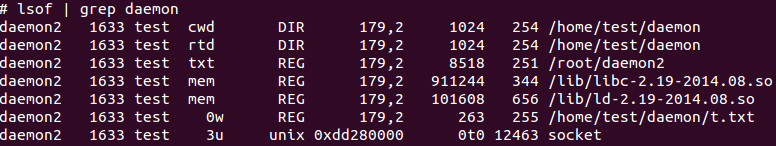
\includegraphics[width=16cm]{daemon_lsof_2.png}
\end{center}
\vspace{0.5cm}

le fichiers \textbf{/var/log/mesages} :

\begin{center} 
\hspace{15cm}
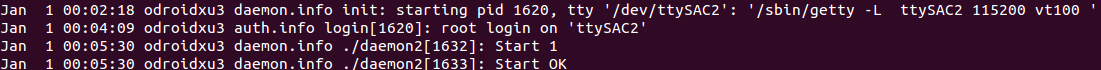
\includegraphics[width=16cm]{daemon_messages_2.png}
\end{center}
\vspace{0.5cm}

ainsi que le fichier \textbf{t.txt} dans lequel il écrit :

\begin{center} 
\hspace{15cm}
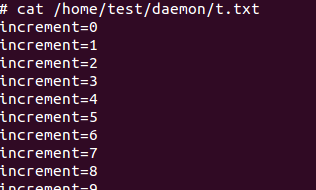
\includegraphics[width=7cm]{daemon_txt_2.png}
\end{center}
\vspace{0.5cm}

Cela nous a permis de savoir que le changement de droits du démon (avec \textbf{umask()}, \textbf{setsid()}, \textbf{setegid()} et \textbf{seteuid()}) fonctionne correctement.

\subsection{Différence entre sysinit et respawn dans inittab}

Dans le fichier \textbf{/etc/inittab} on indique de quelle manière on veut démarrer un démon. Avec \textbf{sysinit} le démon est démarré une seule fois au lors du boot du système. Avec \textbf{respawn} il sera redémarré automatiquement s'il est arrêté.\\

Pour tester la différence entre ces deux modes, on a modifié le fichier \textbf{/etc/inittab} pour y ajouter le démarrage de daemon2, une fois avec \textbf{sysinit} et la seconde avec \textbf{respawn}.\\

\begin{center} 
\hspace{15cm}
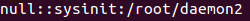
\includegraphics[width=5cm]{daemon_sysinit_inittab.png}
\end{center}
\vspace{0.5cm}

ou :

\begin{center} 
\hspace{15cm}
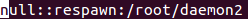
\includegraphics[width=5cm]{daemon_respawn_inittab.png}
\end{center}
\vspace{0.5cm}

Ensuite on redémarre le système avec \textbf{reboot}. Pour \textbf{sysinit} cela donne :

\begin{center} 
\hspace{15cm}
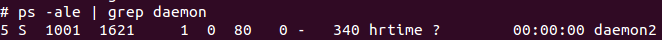
\includegraphics[width=16cm]{daemon_sysinit_ps.png}
\end{center}
\vspace{0.5cm}

\begin{center} 
\hspace{15cm}
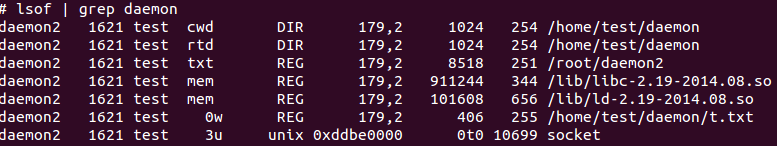
\includegraphics[width=16cm]{daemon_sysinit_lsof.png}
\end{center}
\vspace{0.5cm}

\begin{center} 
\hspace{15cm}
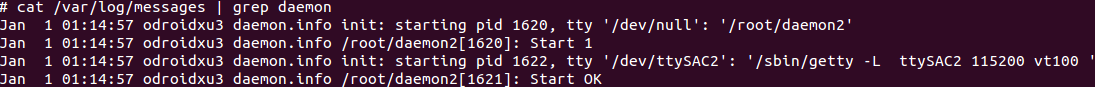
\includegraphics[width=16cm]{daemon_sysinit_messages.png}
\end{center}
\vspace{0.5cm}

\begin{center} 
\hspace{15cm}
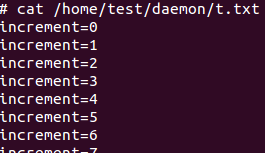
\includegraphics[width=5cm]{daemon_sysinit_txt.png}
\end{center}
\vspace{0.5cm}

On voit donc qu'avec cette technique le démon à démarré et s'est exécuté normalement en même temps que le démarrage du système.

Et pour \textbf{respawn} cela donne :

\begin{center} 
\hspace{15cm}
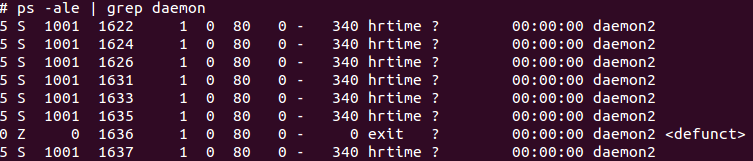
\includegraphics[width=16cm]{daemon_respawn_ps.png}
\end{center}
\vspace{0.5cm}

\begin{center} 
\hspace{15cm}
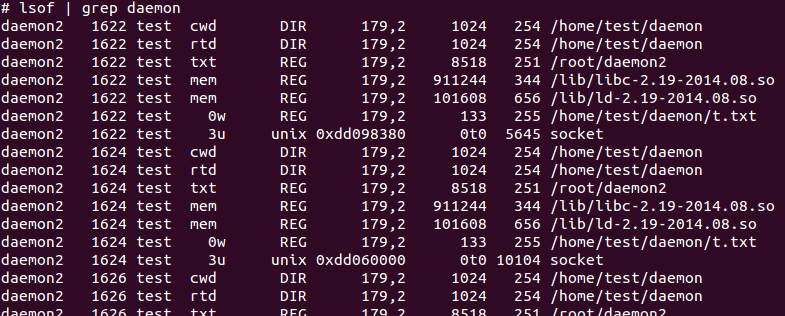
\includegraphics[width=16cm]{daemon_respawn_lsof.png}
\end{center}
\vspace{0.5cm}

\begin{center} 
\hspace{15cm}
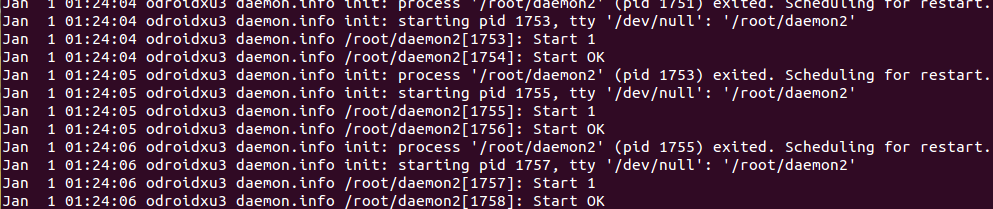
\includegraphics[width=16cm]{daemon_respawn_messages.png}
\end{center}
\vspace{0.5cm}

\begin{center} 
\hspace{15cm}
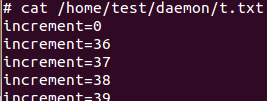
\includegraphics[width=5cm]{daemon_respawn_txt.png}
\end{center}
\vspace{0.5cm}

On voit cette fois qu'il y a plusieurs processus daemon2 qui sont démarrés. Cela est dû au fait que le programme de \textbf{daemon2.c} fait un \textbf{fork()} et que le processus enfant prend le relais alors que le processus parent se termine. Comme le processus parent se termine, le système détecte que le \textbf{daemon2} est terminé et le relance aussitôt puisqu'il est configuré en \textbf{respawn} dans \textbf{inittab}. La nouvelle instance démarre, fait un \textbf{fork()} et etc. le cycle reprend et on obtient une multitude de processus \textbf{daemon2} qui sont lancés...\\

On voit aussi dans le fichier \textbf{t.txt} qu'il ne contient pas des valeurs cohérentes (l'incrément passe d'un coup de 0 à 36). Cela est dû au fait que tous ces processus essaient de d'accéder au fichier de manière concurrente, et y écrivent chacun leur tour avec leur propre valeur d'incrément.

\section{init kernel}
Avant start\_kernel, le processus init démarre les démons nécessaires. 

\section{runlevel}
\begin{lstlisting}[style=Bash]
# Startup the system
null::sysinit:/bin/mount -t proc proc /proc
null::sysinit:/bin/mount -o remount,rw /
null::sysinit:/bin/mkdir -p /dev/pts
null::sysinit:/bin/mkdir -p /dev/shm
null::sysinit:/bin/mount -a
null::sysinit:/bin/hostname -F /etc/hostname
# now run any rc scripts
::sysinit:/etc/init.d/rcS

# Put a getty on the serial port
ttySAC2::respawn:/sbin/getty -L  ttySAC2 115200 vt100 # GENERIC_SERIAL

# Stuff to do for the 3-finger salute
::ctrlaltdel:/sbin/reboot

# Stuff to do before rebooting
::shutdown:/etc/init.d/rcK
::shutdown:/sbin/swapoff -a
::shutdown:/bin/umount -a -r
\end{lstlisting}
Pas de runlevel sous Odroid

sysinit démarre avant toute autre commande telle que boot et bootwait.
